\documentclass{eurodyn2026}
% Loads class "eurodyn2026.cls".

% This class will provide automatically the formatting options required
% The class loads automatically the following packages: hyperref, calc,
% url, graphicx, booktabs, biblatex

\addbibresource{references.bib}

\title{INSTRUCTIONS FOR THE PREPARATION OF FINAL CONTRIBUTIONS FOR THE
XIII INTERNATIONAL CONFERENCE ON STRUCTURAL DYNAMICS (EURODYN 2026)}

\author{First A. Author$^1$, Second B. Author$^2$, and Third C. Author$^2$}

\heading{First A. Author, Second B. Author and Third C. Author}

\address{$^1$Affiliation of First A. Author \\
  address\\
  e-mail: name@e-mail.address \and
  $^2$
  Affiliation of Second B. (and Third C.) Author \\
  address\\
e-mail: \{name2,name3\}@e-mail.address}

\keywords{Keyword 1, Keyword 2, Keyword 3, Keyword 4, Keyword 5, Keyword 6.}

\abstract{This document provides information and instructions for preparing
  papers and extended abstracts to be included in the Proceedings of the XIII International Conference
  on Structural Dynamics (EURODYN 2026). Manuscripts can be written in LaTeX or Word. The first page is reserved for the title, the authors, affiliations, keywords and the abstract. The introduction must begin at the top of the second page.
All the instructions as well as the source for the example files can be found on the conference website.}

\begin{document}

\section{INTRODUCTION}

The proceedings of EURODYN 2026 will be published open access in EASD Procedia. Authors may submit an extended abstract or a full paper. Manuscripts must be written in English within a printing box of 16 cm x 24 cm,
centered in the page. Extended abstracts are between two and four pages including references, figure and tables. Full papers must be at least six pages. There is no restriction on the maximum number of pages for full papers. Note, that only full papers will be indexed in the Scopus database with a link to the full text.

Papers and extended abstracts should be written using the LaTeX or Word templates that can be found on the conference website: \url{https://eurodyn2026.org}, see~\cite{eurodyn2026website}.
\textbf{The file has to be translated to Portable Document Format (PDF) before
submission. Authors must upload the PDF file, correctly formatted, to the submission system}.

The deadline for uploading contributions is given on the conference website. The organizers do not commit themselves to include any paper
received later than this deadline in the proceedings. \textbf{At least one of the authors must register and pay their registration fee before the early bird deadline for their submission to be included in the proceedings and the final program of the conference}.

\section{TITLE, AUTHORS, AFFILIATION, KEYWORDS}

The first page must contain the Title, Author(s), Affiliation(s), Keywords
and the Abstract. The second page must begin with the Introduction. The first
line of the title is located 3 cm from the top of the printing box.

\subsection{Title}

The title should be written centered, in 14pt, boldface Roman, all capital
letters. It should be single spaced if the title is more than one line long.

\subsection{Author}

The author's name should include first name, middle initial and surname. It
should be written centered, in 12pt boldface Roman, 12pt below the title.

\subsection{Affiliation}

Author's affiliation should be written centered, in 11pt Roman, 12pt below
the list of authors. A 12pt space should separate two different affiliations.

\subsection{Keywords}

Please, provide up to six keywords. They should be written left aligned, in 12pt Roman, and the line
must begin with the word \textbf{Keywords:} in boldface. A 30pt space should separate the keywords from the affiliations.

\subsection{Abstract}

Use 12pt Italic Roman for the abstract. The word \textbf{Abstract} must be set
in boldface, not italicized, at the beginning of the first line. The abstract
text should be justified and separated 12pt from the keywords, as shown in the
first page of these instructions. The abstract should neither be too short nor
exceed the first page.

\section{HEADINGS}

Do not use more than two levels of headings. The exact formatting of the section and subsection headings is presented next.

\subsection{Main headings}

The main headings should be written left aligned, in 12pt, boldface and all
capital Roman letters. There should be a 12pt space before and 6pt after the
main headings.

\subsection{secondary headings}

Secondary headings should be written left aligned, 12 pt, boldface Roman, with
an initial capital for first word only. There should be a 12pt space before and
6pt after the secondary headings.

\section{EDITORIAL HEADING}

The first page will include the editorial heading, as shown in the first page
of these instructions. In addition, successive pages will include the name of
the authors. The editorial heading must be included in the paper by the authors.

\section{TEXT}

The normal text should be written single-spaced, justified, using 12pt (Times
New) Roman in one column. The first line of each paragraph must be indented 5mm. There is no inter-paragraph spacing.

\section{PAGE NUMBERS}

The final proceedings will have their own consecutive page numbers, and as a result the authors should \textbf{not} include page numbers in their papers.

\section{FIGURES}

All figures should be numbered consecutively and captioned. The caption title
should be written centered, in 10pt Roman, with upper and lower case letters.

\begin{figure}[ht]
  \begin{center}
    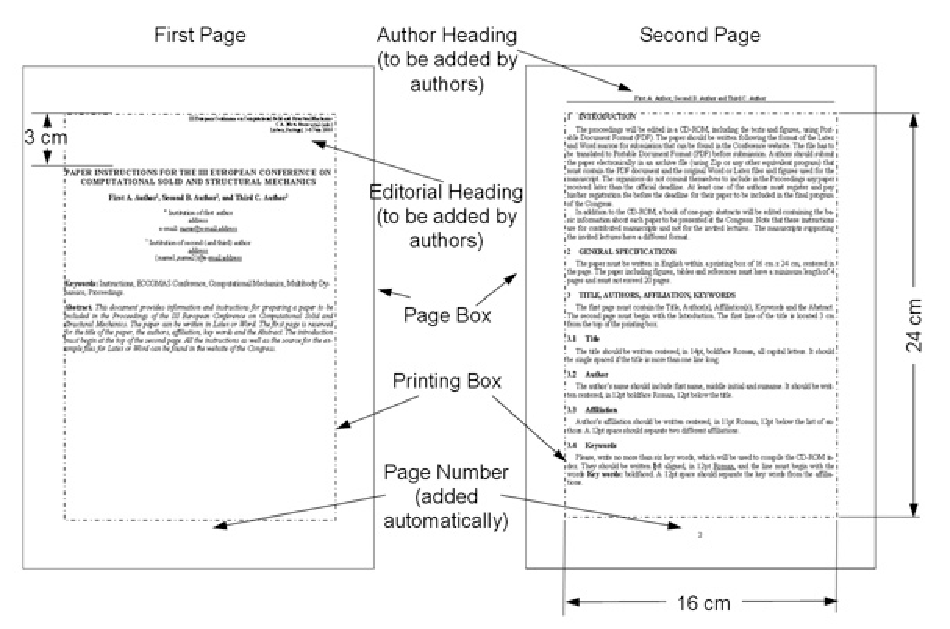
\includegraphics[width=16cm]{figure}
    \caption{Page layout.}
  \end{center}
\end{figure}

A 6pt space should separate the figure from the caption, and a 12pt space should
separate the upper part of the figure and the bottom of the caption from the
surrounding text.

Figures should be included within the text rather than added at the end of the
paper.

\section{EQUATIONS}

A displayed equation is numbered, using Arabic numbers in parentheses. It should
be centered, leaving a 6pt space above and below to separate it from the surrounding
text.

The following example is a single line equation:
\begin{eqnarray}
  Ax = b
\end{eqnarray}

The next example is a multi-line equation:
\begin{eqnarray}
  Ax = b \\
  Bx = c \nonumber
\end{eqnarray}

\section{TABLES}

All tables should be numbered consecutively and captioned, the caption should be 10pt Roman, upper and lower case letters. For horizontal lines use the \texttt{toprule}, \texttt{midrule}, and \texttt{bottomrule} commands provided by the \textit{booktabs} packge. Do \textbf{not} use any vertical lines.

\begin{table}[h]
  \begin{center}
    \begin{tabular}{{ccc}}
      \toprule
      Title 1 & Title 2 & Title 3 \\
      \midrule
      C21     & C22     & C23     \\
      C31     & C32     & C33     \\
      C41     & C42     & C43     \\
      C51     & C52     & C53     \\
      \bottomrule
    \end{tabular}
  \end{center}
  \caption{Example of the construction of one table.}
\end{table}
A 6pt space should separate the table from the caption, and a 12pt space should
separate the table from the surrounding text.

\section{FORMAT OF REFERENCES}

References should be quoted in the text by numbers~\cite{Brown2022,Smith2023,Doe2024}
and grouped together at the end of the paper in numerical order as shown in
these instructions. Three or more consecutive references may be grouped together in the text. The LaTeX template is set up to use \textit{biblatex} and includes  an example bibliography. The section heading of the references should be unnumbered.

\section{CONCLUSIONS}

\begin{itemize}
  \item Papers must be submitted electronically.
  \item Papers must be written following the format of the LaTex or Word
    templates for submission that can be found at the conference website.
  \item Papers must be translated to Portable Document Format (PDF) before
    submission through the submission system.
  \item The deadline for the submission of papers announced on the website must be respected.
  \item The organizers do not commit themselves to include any paper received after the above-mentioned deadline in the proceedings.
  \item At least one of the authors must register and pay their
    registration fee before the early bird  deadline for their paper to
    be included in the final program of the conference and the proceedings.
\end{itemize}

\printbibliography{}

\end{document}
